\section{Waterfall Model}
The waterfall model is a linear and sequential software development approach with distinct phases: requirements gathering, design, implementation, testing, and deployment. It assumes stable requirements but lacks flexibility for changes. It offers structure and milestones but may delay feedback. Suited for projects with stable and well-defined requirements.
\begin{figure}[ht]
    \centering  
    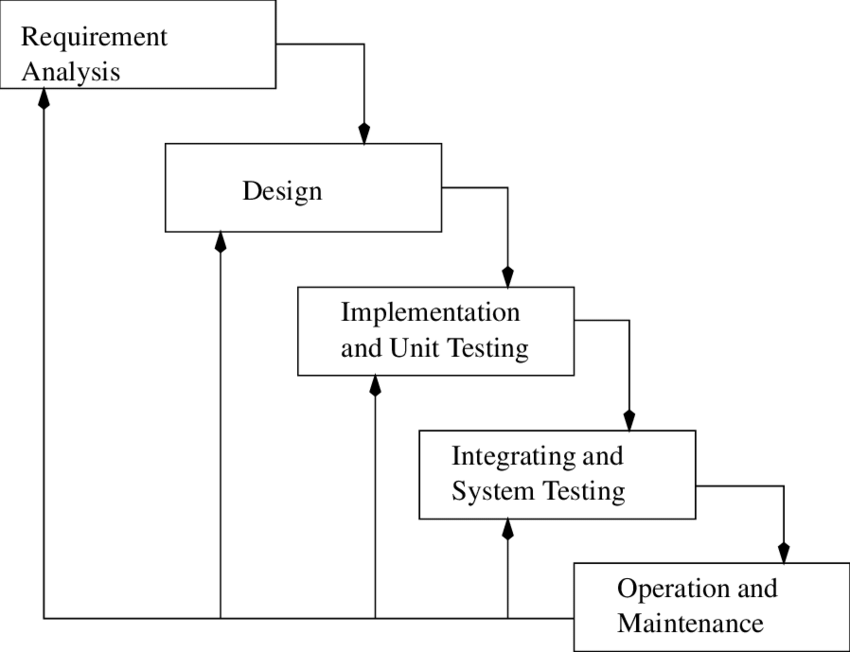
\includegraphics[width=\textwidth, height=0.4\textheight, keepaspectratio]{methodology/model_image/The-Waterfall-Model.png}    
    \caption{Water Fall Model}
    \label{fig:fig 3.6}
\end{figure}